\documentclass[border=2pt]{standalone}
\usepackage{tikz}
\usetikzlibrary{arrows.meta,shapes.symbols}
\begin{document}
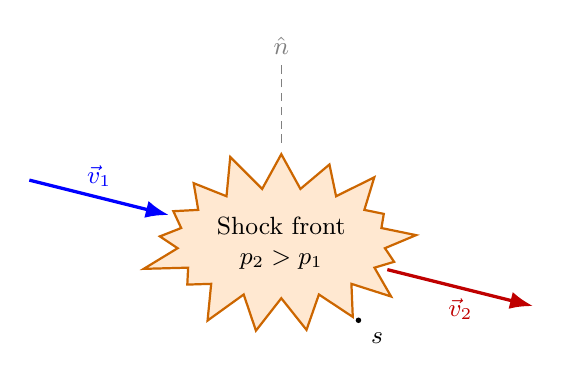
\begin{tikzpicture}[>=Latex,every node/.style={font=\small},
  vector/.style={->,very thick}]
  \node[starburst,starburst points=17,starburst point height=5mm,
    random starburst=2025,minimum width=36mm,minimum height=24mm,
    outer sep=2pt,draw=orange!80!black,fill=orange!18,thick,align=center]
    (shock) {Shock front\\$p_2>p_1$};
  \coordinate (upstream) at (-3.2,.8);
  \coordinate (downstream) at (3.2,-.8);
  \draw[vector,blue] (upstream) -- (shock) node[midway,above] {$\vec v_1$};
  \draw[vector,red!75!black] (shock) -- (downstream) node[midway,below] {$\vec v_2$};
  \draw[densely dashed,gray] (shock.north) -- ++(0,1) node[above] {$\hat n$};
  \fill (shock.south east) circle (1pt) node[below right=1pt] {$s$};
\end{tikzpicture}
\end{document}
